\documentclass[12pt, oneside]{report}

% Packages
\usepackage{graphicx}      % For including images
\usepackage{amsmath, amsfonts, amssymb} % For mathematical symbols and fonts
\usepackage{geometry}      % For page layout
\usepackage{hyperref}      % For hyperlinks
\usepackage{longtable}     % For long tables
\usepackage{cite}          % For citations
\usepackage{fancyhdr}      % For headers and footers
\usepackage{caption, subcaption} % For captions
\usepackage{booktabs}      % For better tables
\usepackage{enumitem}      % For customized lists
\usepackage{algorithm, algorithmic} % For algorithms
\usepackage{tikz, pgfplots} % For graphics
\usepackage{float}         % For improved float placement
\usepackage{setspace}      % For line spacing
\usepackage{listings}      % For code listings

% Page setup
\geometry{left=1in, right=1in, top=1in, bottom=1in} % Define page margins

\hypersetup{
    colorlinks=true,
    linkcolor=blue,
    filecolor=magenta,
    urlcolor=cyan,
}

\pagestyle{fancy}
\fancyhf{}
\fancyhead[L]{AFQ-IoT : Adaptive,Federated and Quantum-Resistant AI-Blockchain IoT Framework}
\fancyhead[R]{\thepage}
\renewcommand{\headrulewidth}{0.4pt}

% Fix fancyhdr headheight warning
\setlength{\headheight}{15pt}

% Set pgfplots compatibility
\pgfplotsset{compat=1.18}

\begin{document}

% Custom Title Page
\begin{titlepage}
    \centering
    \vspace*{1cm} % Adjust vertical space from the top of the page
    
    % Institution Logo
    
\includegraphics[width=0.4\textwidth]{img.jpg} \\[1cm] % Adjust width as needed
    
    % Project Title
    {\Huge\textbf{AFQ-IoT}}\\[0.5cm]
    {\Large A Blockchain-enabled Intelligent IoT Architecture with Artificial Intelligence}\\[1cm]
    
    % Project Details
    {\Large\textbf{Research in Information Security}}\\[0.3cm]

    
    % Team Information
    {\Large\textbf{Team Number :10}}\\[0.5cm]
    \begin{tabular}{|c|c|c|}
    \hline
    \textbf{Team Member} & \textbf{Roll Number} & \textbf{Program of Study} \\
    \hline
    Shiva Shankar & 2023202005 & CSIS \\
    Akshay Kohad & 2023202007 & CSIS \\
    Ashish Lakhmani & 2023202008 & CSIS \\

    \hline
    \end{tabular}\\[1cm]
    
    % Submission Date
    {\Large Submission Date: November 5, 2024}
    
    \vfill % Pushes the content to the top and bottom
    
    % Optional Footer or Additional Information
    % You can add your advisor's name or institution here if needed
\end{titlepage}

% Abstract

\section*{Abstract}
The Internet of Things (IoT) is used in a wide range of applications, such as smart cities, healthcare, and transportation, for the betterment of human life. However, IoT networks produce a lot of data, which needs to be processed in an efficient, scalable, and real-time manner. Most of the traditional centralized architecture suffers from problems related to data security, privacy, scalability, and latency. Hence, to overcome these, this paper proposes an AFQ-IoT framework advanced, adaptive IoT architecture.
that extends and builds upon the BlockIoTIntelligence model. Federated learning, quantum-resistant blockchain, cross-chain interoperability, and adaptive AI-driven consensus enable AFQ-IoT to ensure secure, decentralized data handling and efficient analytics across device, edge, fog, and cloud intelligence layers. As core technologies, "AI-enhanced Blockchain" and "Blockchain-secured AI" allow AFQ-IoT to support real-time, context-aware decision-making and inter-domain data sharing while future-proofing IoT networks against quantum threats. 

% Keywords
\section*{Keywords}
\noindent \textbf{Internet of Things (IoT), Blockchain, Artificial Intelligence (AI), Decentralized Architecture,Adaptive Learning, Federated Learning, Quantum Resistant}
   



% Table of Contents
\tableofcontents
\newpage

% List of Figures
\listoffigures
\addcontentsline{toc}{chapter}{List of Figures}
\newpage

% List of Tables
\listoftables
\addcontentsline{toc}{chapter}{List of Tables}
\newpage

% Section 1: Introduction
\chapter{Introduction}

\section{Background}
% Background content goes here.
The report introduces the "Internet of Things" concept and its framework that unifies different
peripherals, enabling seamless communication among devices. This connection extends ap-
The applications extend to smart homes, transportation, and automotive systems. Even though
These disadvantages are also faced by IoT regarding big data analytics, security, privacy, and latency.
due to its centralized architecture, which limits efficiency in handling large-scale data. The
The proposed solution explores integrating Blockchain for decentralization and Artificial Intelli-
gence or AI for data processing and analysis, solving the present challenges to make IoT much more
scalable and secure.
\section{Network Model}
% Define network model here.
The network model in this proposed architecture consists of a multi-layered structure involving mainly 4 components: 

\begin{itemize}
    \item \textbf{Device intelligence} - Consists of various IoT devices with AI and blockchain applications; it produces a massive amount of data, which is transferred to the edge intelligence.
    \item \textbf{Edge intelligence} - Consists of AI-enabled base stations connected to the blockchain at the edge of the network.The process data from edge intelligence are reported to the fog intelligence, which is a combination of several AI-enabled fog nodes with Blockchain.
    \item \textbf{Fog intelligence} - Consists of multiple AI-enabled fog nodes that also utilize blockchain. The fog nodes provide an intermediate processing layer between the edge and the cloud.
    \item \textbf{Cloud intelligence} - consists of AI-enabled data centers that are connected to the blockchain to provide decentralized and secure big data of IoT applications such as smart healthcare, smart transportations etc.
\end{itemize} 
\begin{figure}[H] % 'H' places the image exactly here, using float package
    \centering
    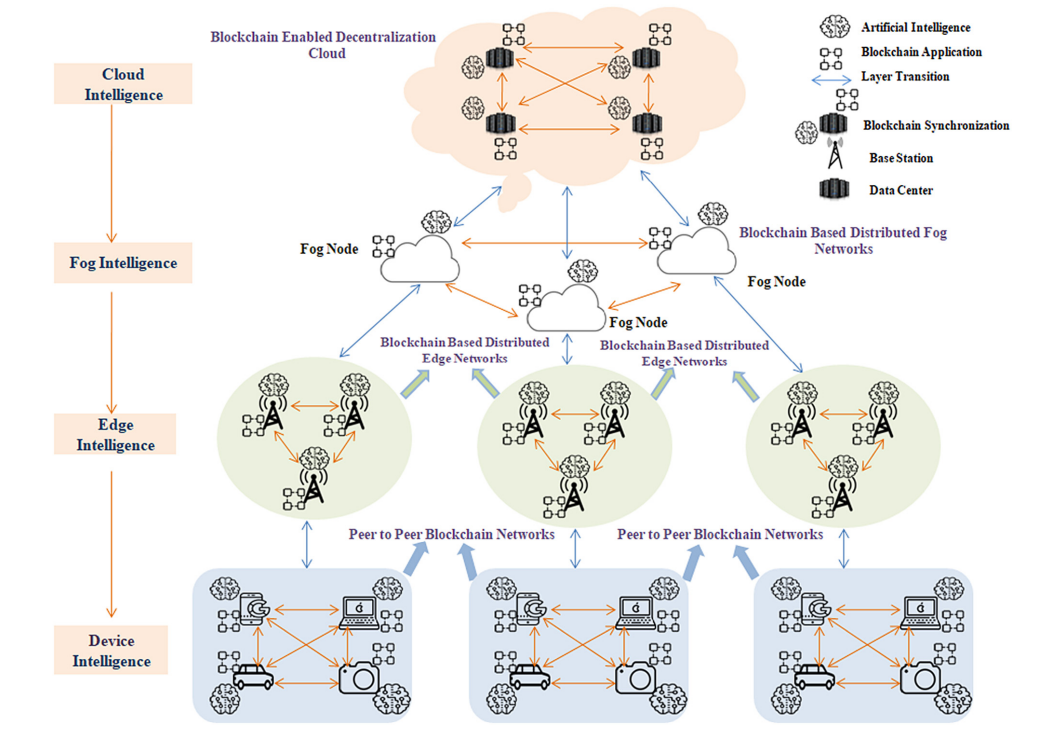
\includegraphics[width=0.7\textwidth]{BlockChainIOT.png} % Adjust width as needed
    \caption{Network Model of BlockIoTIntelligence Architecture} % Add a relevant caption
    \label{fig:network_model} % Label for referencing
\end{figure}

Each Intelligence is created to analyze data at different levels, which would support efficient data
In handling and security, blockchain technology is used to decentralize control, and AI is
Incorporated for the real-time analysis of data, form a networked system, where information flows
Safety of IoT devices at the edge, fog, and cloud Intelligence.
 
\section{Attack Model}
% Define attack model here.
The Attack Model is specifically operational in Fog Intelligence.The model utilizes a decentralized security architecture based on blockchain,artificial intelligence, and software-defined networking (SDN) to analyze incoming IoT data for potential attacks. Ethereum blockchain technology is implemented to deliver a decentralized approach to big data analysis, aiming to mitigate centralization issues. The system supports attack detection at the fog node, addressing storage, computation, and latency constraints effectively. Performance parameters include accuracy, detection rate, computational resources, and more. This architecture reportedly offers an efficient way to counter attacks in smart IoT networks, such as smart transportation systems.
% \section{Research Contributions}
% State your research contributions here.
\section{Research Contributions}

The \textbf{AFQ-IoT Framework} introduces a novel approach to addressing key challenges in the Internet of Things (IoT) by integrating adaptive AI-driven methods, federated learning, quantum-resistant cryptography, and cross-chain interoperability. The primary research contributions of this work are as follows:

\begin{itemize}

    \item \textbf{Privacy-Preserving Federated Learning for IoT Devices}: 
    It has federated learning at the device layer, and it is possible to do on-device AI model training while keeping raw data local. This helps reduce privacy risks and minimize data transmission, thereby making the framework suitable for privacy-sensitive applications such as healthcare and finance.

    \item \textbf{Quantum-Resistant Cryptographic Security}: 
    AFQ-IoT integrates quantum-resistant cryptographic algorithms that keep IoT data and transactions secure against future threats arising from the advent of future quantum computing capabilities. It readies the IoT architecture for the quantum computing era and has long-term protection for data.

    \item \textbf{Adaptive Consensus Mechanism for Efficient Resource Utilization}: 
    The framework introduces an AI-driven adaptive consensus mechanism at the cloud layer, which switches dynamically based on network load and security needs. AFQ-IoT will be optimized in terms of energy consumption and computation so that the system is scalable and sustainable for resource-constrained IoT environments.

    \item \textbf{Cross-Chain Compatibility for Multi-Domain Interoperability}: 
   AFQ-IoT supports cross-chain interoperability at the fog layer with protocols such as Polkadot and Cosmos. This will enable secure and efficient data exchange among various IoT domains, for instance, healthcare, transportation, and industrial IoT. It will support complex multi-domain IoT applications, including smart city and emergency response systems.

    \item \textbf{Localized Blockchain and Distributed AI for Enhanced Edge Processing}: 
    The framework localizes blockchain and distributed AI models at the edge layer to support decentralized data handling and provide local processing capabilities. Real-time, context-aware decision-making at the edge layer will be possible with less latency while making systems more responsive in dynamic IoT environments.

    \item \textbf{Federated Trust Mechanism for Secure Collaborative Anomaly Detection}: 
    A federated trust mechanism supports collaborative anomaly detection and validation of data across IoT layers and devices. This has the effect of improving the security of the system with decentralized trust and resilience in the face of attacks. It does this by distributing both data validation and threat detection throughout the network.

    \item \textbf{Energy-Efficient Quantized AI Models for Scalable Large-Scale Analysis}: 
    Such cloud-layer AI models are designed with the strategy of quantization, which has a relatively low energy consumption but reduces computation complexity. In other words, it enables the analysis of large data and is affordable for an IoT system with scarce resources.

\end{itemize}

In summary, the AFQ-IoT Framework offers a comprehensive and forward-looking IoT solution by addressing the challenges of privacy, security, scalability, and interoperability through innovative AI and blockchain techniques. This framework is well-suited for modern IoT applications and prepares for emerging technological challenges, including quantum computing and multi-domain IoT integration.

% Section 2: Literature Review
\chapter{Literature Review}

\section{Related Works}
% Discuss related works here.
\begin{itemize}
\item \textbf{Blockchain and AI Integration:} Researchers have proposed using Blockchain’s decentralized structure to overcome centralization and security issues in IoT. The AI component is applied for data analysis and decision-making, especially for large datasets generated by IoT devices.

\item \textbf{Architectural Solutions:} Solutions are categorized into cloud, fog, edge, and device layers. For example, fog computing enables distributed data processing closer to IoT devices, mitigating latency issues. Blockchain is deployed at multiple layers to enhance security and decentralization, while AI assists with data processing at each layer.

\item \textbf{Evaluation Metrics:} The studies evaluate IoT systems on factors like accuracy, latency, security, computational complexity, and energy efficiency. These metrics are used to compare the efficacy of various architectures and techniques.

\end{itemize}

The related works discussed in the research paper cover various approaches to integrating Blockchain, Artificial Intelligence (AI), and the Internet of Things (IoT), with each study contributing unique insights into this convergence.

\begin{enumerate}
\item \textbf{Rathore et al. (2019)\cite{rathore2019}}
\begin{itemize}
    \item \textbf{Technological Aspect}: Blockchain + AI
    \item \textbf{Focus}: Presented a secure deep learning framework integrating Blockchain with AI to address data security issues in IoT applications. Blockchain ensures a tamper-resistant environment, while deep learning techniques improve data analysis accuracy, enhancing the trustworthiness and reliability of data generated by IoT devices.
\end{itemize}

\item \textbf{Atlam et al. (2018)\cite{atlam2018}}
\begin{itemize}
    \item \textbf{Technological Aspect}: IoT + AI
    \item \textbf{Focus}: Provided a comprehensive overview of integrating AI and IoT, emphasizing benefits and potential challenges. Highlighted AI's role in enhancing decision-making processes within IoT applications, improving data analysis, anomaly detection, and operational efficiency. Also explored limitations and opportunities arising from integrating AI with IoT infrastructure.
\end{itemize}

\item \textbf{Wright et al. (2018)\cite{wright2018}}
\begin{itemize}
    \item \textbf{Technological Aspect}: Blockchain + IoT + Edge Computing
    \item \textbf{Focus}: Introduced an Ethereum-based smart edge computing solution for efficient resource management within IoT systems. This framework enables nodes to offload computational tasks to edge devices in exchange for payments, optimizing computational resources, reducing latency, and lowering costs.
\end{itemize}

\item \textbf{Zheng et al. (2017)\cite{zheng2018}}
\begin{itemize}
    \item \textbf{Technological Aspect}: Blockchain
    \item \textbf{Focus}: Zheng et al. created a detailed taxonomy of Blockchain technology, breaking down its key characteristics, consensus algorithms, applications, and the technical challenges it faces. This taxonomy serves as a foundational guide for understanding how Blockchain can support IoT by enhancing data security and decentralization. By analyzing the strengths and limitations of Blockchain, the study offers insights into its potential role in managing IoT data.
\end{itemize}


\item \textbf{Qian et al. (2018)\cite{qian2018}}
\begin{itemize}
    \item \textbf{Technological Aspect}: Blockchain + IoT
    \item \textbf{Focus}: Proposed a Blockchain-based security management system for IoT, enhancing data security by enabling Blockchain for abnormal traffic monitoring and identity verification. This approach mitigates security vulnerabilities within IoT, particularly in monitoring network anomalies and ensuring authorized device access.
\end{itemize}


\item \textbf{Xu et al. (2017)\cite{xu2017}}
\begin{itemize}
    \item \textbf{Technological Aspect}: Blockchain + AI
    \item \textbf{Focus}: Developed a decentralized resource management framework based on Blockchain and AI, aimed at optimizing energy usage in IoT applications. This approach is particularly useful for energy-efficient IoT systems where resource allocation is critical.
\end{itemize}


\item \textbf{Vukobratovic et al. (2016)\cite{vukobratovic2016}}
\begin{itemize}
    \item \textbf{Technological Aspect}: AI + IoT
    \item \textbf{Focus}: This study proposed a reconfigurable knowledge acquisition system for IoT, incorporating network function virtualization and machine learning. The system enhances data analysis capabilities within IoT, allowing for efficient and scalable data processing. By integrating AI with IoT, the study demonstrates how machine learning can optimize IoT data collection and processing for various applications.
\end{itemize}
\end{enumerate}


\section{Summary of Techniques}
% Provide a table summarizing techniques, advantages, and disadvantages.

\begin{longtable}{|p{3.5cm}|p{3.5cm}|p{3.5cm}|p{3.5cm}|}
\hline
\textbf{Research Work} & \textbf{Techniques Used} & \textbf{Advantages} & \textbf{Disadvantages} \\
\hline
\endfirsthead

\hline
\textbf{Research Work} & \textbf{Techniques Used} & \textbf{Advantages} & \textbf{Disadvantages} \\
\hline
\endhead

\hline
\endfoot

% Table Content
Rathore et al. \cite{rathore2019} & Blockchain + AI & Improved security for IoT data & Limited scalability \\
\hline
Atlam et al. \cite{atlam2018} & IoT + AI & Enhanced decision-making capabilities & High computational cost \\
\hline
Wright et al. \cite{wright2018} & Ethereum-based smart contracts & Low-cost resource management & Limited to specific edge-computing environments \\
\hline
Zheng et al. \cite{zheng2018} & Blockchain taxonomy and consensus algorithms & Distributed security & Complexity in implementation \\
\hline
Qian et al. \cite{qian2018} & Blockchain + IoT & Improved data integrity and anomaly detection & Limited real-time application \\
\hline
Xu et al. \cite{xu2017} & Blockchain-based resource management & Optimized energy usage in IoT & Limited decision-making flexibility \\
\hline
Vukobratovic et al. \cite{vukobratovic2016} & AI + IoT & Enhanced data analysis and scalability & Hardware dependency \\
\hline

% Add more rows as needed
\end{longtable}


% Section 3: Your Proposal
\chapter{Your Proposal}

\section{Motivation}
% Discuss the motivation behind your proposal.
The paper "\textbf{BlockIoTIntelligence: A Blockchain-enabled Intelligent IoT Architecture with Artificial Intelligence}" Proposes an architecture that integrates blockchain and AI to address some of the most significant IoT challenges in terms of centralization, security, and latency. The proposed architecture demonstrates some tremendous advancements, yet many issues and challenges are left untouched, including energy efficiency, interoperability, data management, and privacy-preserving AI. These limitations are a clear motivation for further research on extending the framework towards more adaptive, sustainable, and privacy-focused BlockIoTIntelligence for real-world IoT applications.

Our proposal aims to address these gaps by enhancing the BlockIoTIntelligence architecture by introducing new Architecture called AFQ-IoT.

\section{Introduction to Adaptive, Federated, and Quantum-Resistant AI-Blockchain IoT Framework (AFQ-IoT)}
The \textbf{AFQ-IoT} framework is an evolution of the BlockIoTIntelligence architecture, which integrates federated learning, adaptive consensus mechanisms, lightweight blockchain, cross-chain interoperability, and quantum-resistant cryptography in a layered approach. The framework provides a secure, scalable, and collaborative environment for IoT applications and is flexible enough to be adapted to unique needs in different fields, such as healthcare, transportation, and industrial IoT.
Our proposal, therefore addresses these gaps with proposing the AFQ-IOT architecture by:

\begin{itemize}
    \item \textbf{Federated Learning for Privacy and Efficiency} reduces data transfer and maintains privacy by keeping sensitive information on IoT devices, addressing privacy and bandwidth limitations in centralized models.


    \item \textbf{Adaptive AI-Driven Consensus Mechanism} balances security with energy efficiency by switching consensus protocols based on network load, solving the energy inefficiencies of fixed consensus mechanisms in IoT.
    \item \textbf{Cross-Chain Compatibility for Interoperability} enables secure, real-time data exchange across multiple IoT domains, eliminating data silos and enhancing interoperability in multi-domain applications.
    \item \textbf{Quantum-Resistant Cryptography for Future-Proof Security} protects IoT transactions from quantum attacks, ensuring long-term security for sensitive data and overcoming the vulnerability of traditional cryptography.

    \item \textbf{Adaptive AI Models} provides responsive decision-making by dynamically adjusting to changing data patterns, which enhances accuracy and reduces latency in IoT applications with evolving conditions.
   
\end{itemize}
\section{Proposed Solution}
% Describe your proposed solution here.
Our enhanced proposal builds upon the original BlockIoTIntelligence architecture by addressing specific limitations in energy efficiency, privacy, interoperability, and data management. The key components of this proposal include:


\begin{enumerate}
    \item \textbf{Federated Learning for Privacy and Efficiency}:
    \begin{itemize}
        \item \textbf{Objective}: Preserve data privacy while reducing communication overhead in IoT networks. Due to this, it minimizes energy consumption associated with blockchain operations in IoT networks.
        \item \textbf{Approach}: Use federated learning to train AI models locally on IoT devices, sharing only model updates instead of raw data.
        \item \textbf{Justification}: Traditional centralized AI models require transmitting raw data, raising privacy concerns and increasing bandwidth usage. Federated learning minimizes data transfer and keeps sensitive information on devices, essential for privacy-sensitive applications like healthcare.
    \end{itemize}
    
    \begin{figure}[h!]
        \centering
        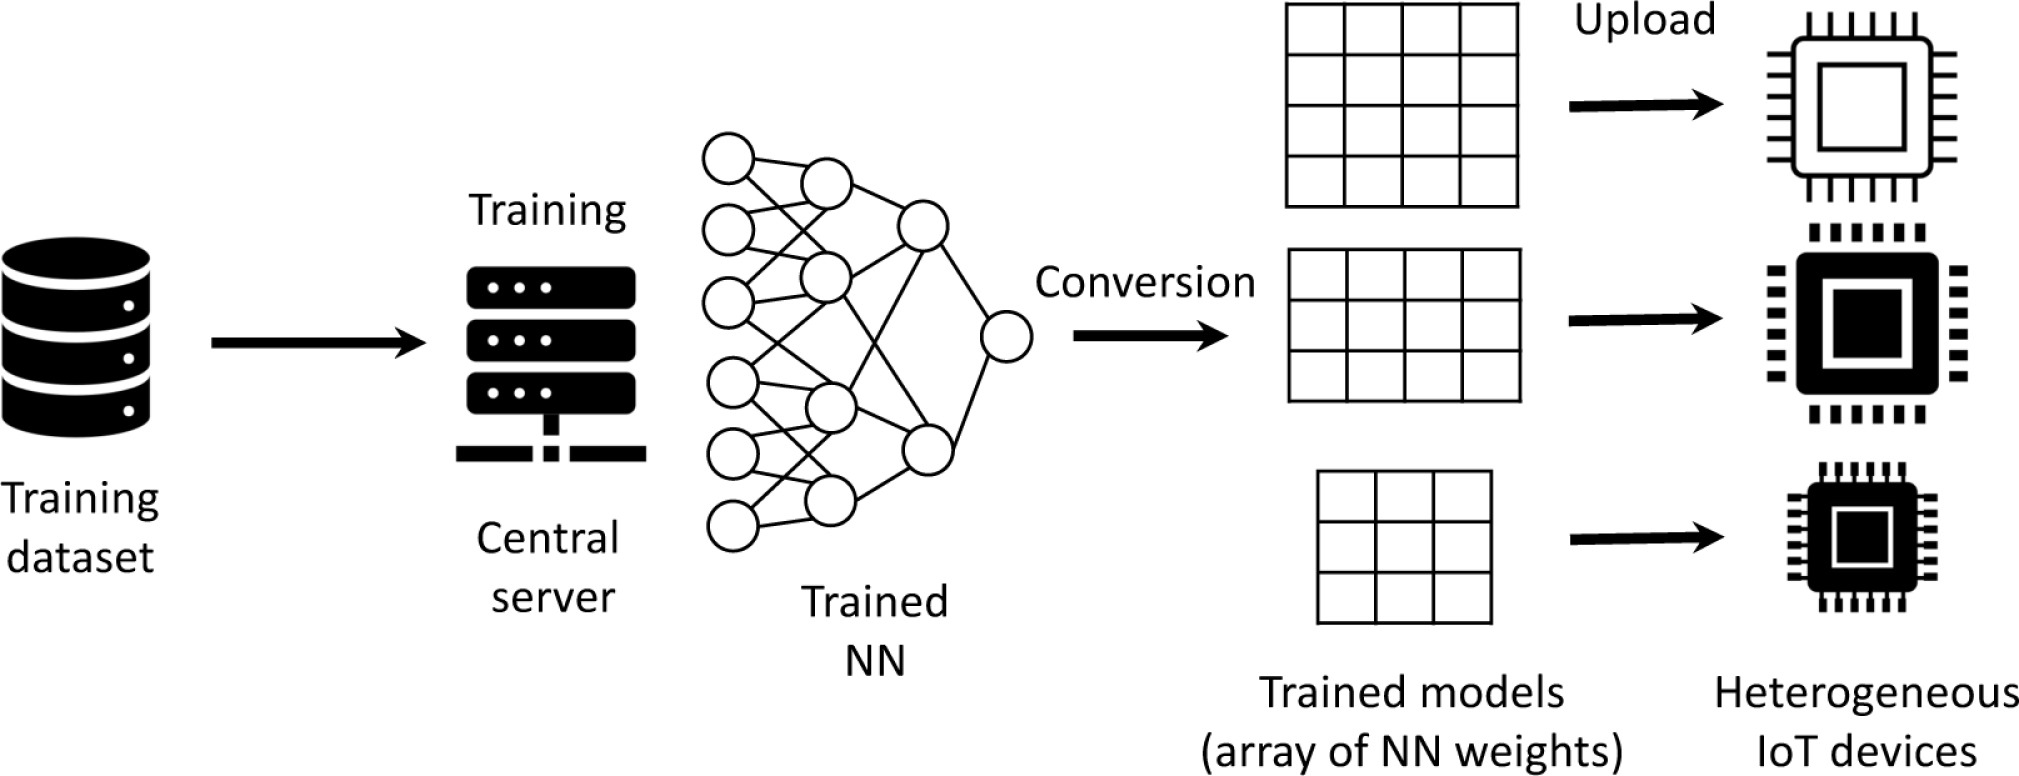
\includegraphics[width=0.45\textwidth]{trad.jpg}
        \caption{Example of federated learning workflow in IoT networks \cite{ficco2023}.}
        \label{fig:Traditional model training process.}
    \end{figure}

    \begin{figure}[h!]
        \centering
        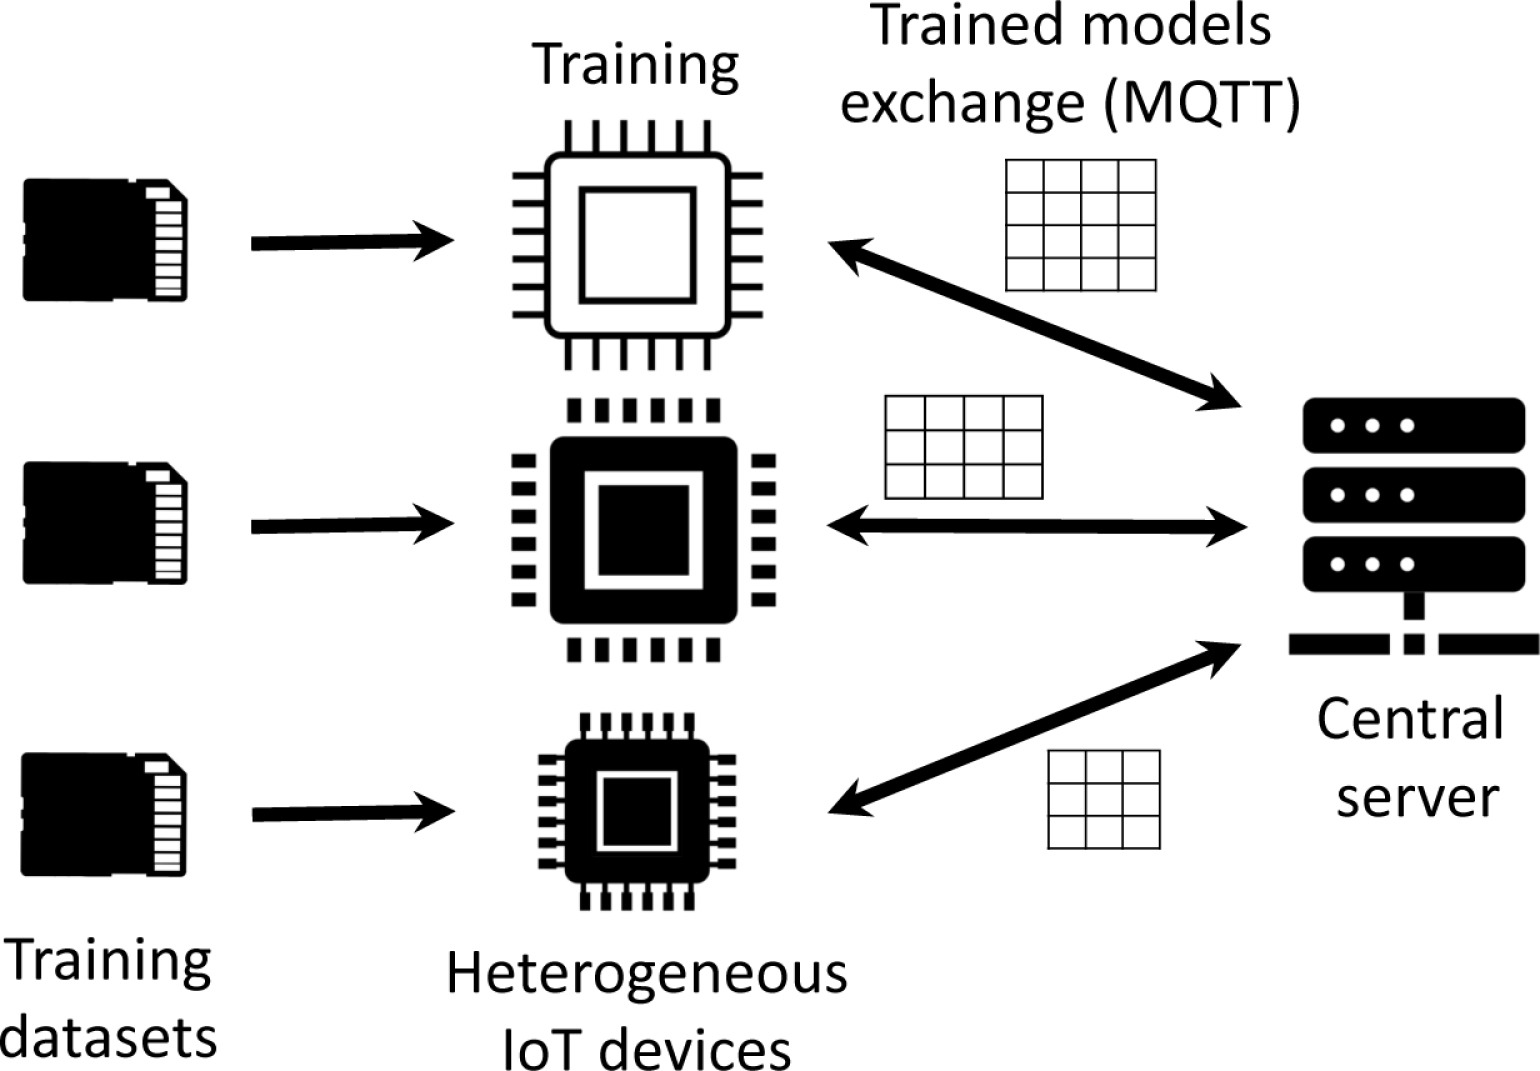
\includegraphics[width=0.45\textwidth]{fed.jpg}
        \caption{Energy efficiency improvements through federated learning \cite{ficco2023}.}
        \label{fig:collaborative training process}
    \end{figure}


    \item \textbf{Adaptive AI-Driven Consensus Mechanism for Security and Resource Optimization}:
    \begin{itemize}
        \item \textbf{Objective}: Balance security needs with energy efficiency based on network load and conditions.
        \item \textbf{Approach}: Implement an adaptive consensus protocol that switches between Proof-of-Stake (PoS) and Proof-of-Authority (PoA) depending on network demands.
        \item \textbf{Justification}: Fixed consensus mechanisms (e.g., PoW) consume significant energy and are unsuitable for resource-constrained IoT devices. An adaptive mechanism optimizes resource usage and enhances security only when needed, making it more efficient for fluctuating network conditions.
    \end{itemize}

    \item \textbf{Cross-Chain Compatibility for Interoperability}:
    \begin{itemize}
        \item \textbf{Objective}: Enable secure data sharing across different IoT domains (e.g., healthcare, transportation) without compromising domain-specific security needs.
        \item \textbf{Approach}: Integrate cross-chain protocols (e.g., Polkadot, Cosmos) at the fog layer to facilitate inter-domain communication.
        \item \textbf{Justification}: Single-chain systems limit interoperability, creating data silos in multi-domain IoT applications. Cross-chain compatibility allows secure, flexible interactions across domains, essential for applications like emergency response systems where diverse data sources must collaborate in real-time.
    \end{itemize}

    \item \textbf{Quantum-Resistant Cryptography for Future-Proof Security}:
    \begin{itemize}
        \item \textbf{Objective}: Protect IoT data and transactions from future quantum-based attacks.
        \item \textbf{Approach}: Use quantum-resistant cryptographic algorithms, such as lattice-based cryptography, within the blockchain framework.
        \item \textbf{Justification}: Traditional cryptography is vulnerable to quantum computing advancements, which could compromise data security. Quantum-resistant cryptography ensures long-term data protection, crucial for applications requiring persistent data security, such as financial and healthcare IoT.
    \end{itemize}


    \item \textbf{Adaptive AI Models for Real-Time Decision Making}:
    \begin{itemize}
        \item \textbf{Objective}: Enhance real-time responsiveness and decision-making in IoT applications.
        \item \textbf{Approach}: Adaptive machine learning models could use reinforcement learning up to transfer learning. Using them requires dynamic adjustment in terms of changes in the network environments and data patterns. Establishing faster responses for IoT traffic management or predictive maintenance might be possible.
        \item \textbf{Justification}: IoT applications often require rapid adjustments to new data. Adaptive AI models allow the system to respond promptly, improving decision accuracy and reducing latency.
    \end{itemize}
\end{enumerate}
\subsection{Key Components and Design}

The AFQ-IoT architecture has five primary layers, each responsible for specific tasks while ensuring security, privacy, and adaptability in IoT environments:

\begin{enumerate}
    \item \textbf{Device Intelligence Layer with Federated Learning and Quantum-Resistant Lightweight Blockchain}:
    \begin{itemize}
        \item \textbf{Federated Learning for Privacy}: Each IoT device trains its local AI model on-device data to prevent unnecessary data transmission. Federated learning enables collaborative AI model improvement without centralizing raw data, which preserves privacy and reduces bandwidth consumption.
        \item \textbf{Quantum-Resistant Lightweight Blockchain}: Given the resource limitations of IoT devices, a lightweight blockchain structure with quantum-resistant cryptography (e.g., lattice-based algorithms) is employed. This blockchain records key transactional data while maintaining a small footprint to accommodate the limited computational capabilities of devices.
        \item \textbf{Functionality}: This layer performs initial data processing and filtering. Only necessary model updates (rather than data) are shared with higher layers, ensuring minimal data transfer while preserving privacy and energy efficiency.
    \end{itemize}

    \item \textbf{Edge Intelligence Layer with Adaptive AI Models and Localized Blockchain}:
    \begin{itemize}
        \item \textbf{Adaptive AI Models}: This layer includes edge nodes (like local servers or powerful IoT hubs) capable of more intensive data analysis and processing. Adaptive AI models at the edge layer dynamically adjust based on context, device type, and data type, providing real-time analysis and pattern recognition for immediate decision-making.
        \item \textbf{Localized Blockchain for Edge Security}: A localized blockchain ledger is deployed to record interactions between edge nodes and IoT devices, ensuring data integrity and authentication without requiring constant interaction with the main cloud. Smart contracts automate data verification, access control, and anomaly detection within the local network.
        \item \textbf{Functionality}: The edge layer consolidates filtered data from the device layer, processes it for relevant patterns (e.g., identifying traffic congestion or potential anomalies), and determines which data should be shared with the fog and cloud layers. It provides both security and privacy controls, enabling near real-time responses for critical applications.
    \end{itemize}

    \item \textbf{Fog Intelligence Layer with Dynamic Cross-Chain Compatibility}:
    \begin{itemize}
        \item \textbf{Cross-Chain Compatibility}: This layer incorporates cross-chain capabilities, allowing various IoT sub-networks (e.g., healthcare, logistics, energy) to interoperate. Using protocols like Polkadot or Cosmos, it enables secure data exchange between different blockchain environments without compromising the specialized features of each chain.
        \item \textbf{Distributed AI for Resource Management}: AI-driven resource management optimizes bandwidth allocation and computing power, balancing the load across networks. This is crucial for environments where data demand fluctuates, like industrial IoT networks or smart city infrastructure.
        \item \textbf{Functionality}: The fog layer manages data interactions between the edge and cloud, focusing on inter-domain data exchanges. For instance, healthcare IoT data can interact with transportation data securely, enhancing applications like emergency response where cross-domain data is valuable.
    \end{itemize}

    \item \textbf{Cloud Intelligence Layer with AI-Driven Consensus and Quantized AI Models}:
    \begin{itemize}
        \item \textbf{AI-Driven Adaptive Consensus}: At the cloud layer, the blockchain uses an AI-driven consensus mechanism that dynamically adjusts based on network demands. For instance, it can switch from Proof-of-Authority (PoA) during low activity to Proof-of-Stake (PoS) during high-activity periods, optimizing security and reducing energy consumption.
        \item \textbf{Quantized AI Models for Efficiency}: Cloud servers handle large-scale data analysis using quantized AI models that reduce computational load. Quantization makes it feasible to analyze massive IoT datasets without overwhelming processing resources, offering scalable solutions that maintain accuracy.
        \item \textbf{Functionality}: The cloud layer is the centralized, high-power processing unit for handling long-term, large-scale analytics and coordination between layers. It also serves as the main data storage, protected by secure consensus protocols and automated AI security monitoring.
    \end{itemize}

    \item \textbf{Security and Privacy Management Layer with Federated Trust and Quantum-Resistant Smart Contracts}:
    \begin{itemize}
        \item \textbf{Federated Trust and Anomaly Detection}: A federated trust mechanism across devices, edge, and cloud layers ensures that data from all layers is validated by smart contracts. This decentralized trust system facilitates real-time anomaly detection and device authentication, securing against cyber threats.
        \item \textbf{Quantum-Resistant Smart Contracts for Access Control}: Quantum-resistant smart contracts control access to sensitive data, making use of advanced cryptographic algorithms like lattice-based cryptography. These smart contracts enforce policies based on predefined rules, such as only allowing verified healthcare providers to access patient data.
        \item \textbf{Functionality}: This layer integrates with all other layers to ensure robust security and privacy, using federated trust mechanisms to validate data while smart contracts automate access control and data integrity verification across the network.
    \end{itemize}
\end{enumerate}


\begin{table}[h!]
\centering
\resizebox{\textwidth}{!}{%
\begin{tabular}{|p{4cm}|p{5cm}|p{5cm}|p{5cm}|}
\hline
\textbf{Layer} & \textbf{AFQ-IoT Framework (Proposed)} & \textbf{BlockIoTIntelligence} & \textbf{Key Differences} \\
\hline
\textbf{Device Intelligence Layer} & 
- \textbf{Federated Learning} for privacy-preserving model training on-device. \newline 
- \textbf{Quantum-resistant lightweight blockchain} for secure transactions at minimal computational cost. \newline 
- Initial data filtering and minimal data transmission. & 
- Uses a traditional blockchain for secure data handling. \newline 
- AI performs basic data filtering but no federated learning. & 
\textbf{Federated Learning} enables privacy-preserving training; \textbf{quantum-resistant blockchain} offers enhanced security for future-proofing. \\
\hline
\textbf{Edge Intelligence Layer} & 
- \textbf{Adaptive AI Models} for real-time processing and pattern recognition. \newline 
- \textbf{Localized Blockchain} for managing local data integrity and access through smart contracts. & 
- AI is used for local data processing without adaptability based on context. \newline 
- Relies on centralized data verification. & 
\textbf{Adaptive AI} provides flexibility, while \textbf{localized blockchain} ensures efficient, decentralized data handling. \\
\hline
\textbf{Fog Intelligence Layer} & 
- \textbf{Cross-Chain Compatibility} with protocols like Polkadot or Cosmos, enabling inter-domain data sharing securely. \newline 
- \textbf{Distributed AI} for resource and load management, ensuring network efficiency. & 
- No cross-chain compatibility; operates within a single blockchain domain. \newline 
- Basic load distribution without resource optimization. & 
\textbf{Cross-chain compatibility} allows interoperability across domains; \textbf{distributed AI} improves resource management. \\
\hline
\textbf{Cloud Intelligence Layer} & 
- \textbf{AI-Driven Adaptive Consensus} that dynamically switches protocols based on network load and security needs. \newline 
- \textbf{Quantized AI Models} reduce computational costs for large-scale analysis. & 
- Uses a standard blockchain consensus (Proof-of-Work or similar) without adaptability. \newline 
- Full-sized AI models without quantization. & 
\textbf{Adaptive consensus} optimizes energy use, and \textbf{quantized AI models} improve scalability for large IoT deployments. \\
\hline
\textbf{Security and Privacy Layer} & 
- \textbf{Federated Trust Mechanism} for collaborative anomaly detection and data validation. \newline 
- \textbf{Quantum-Resistant Smart Contracts} for access control and data protection. & 
- Centralized trust model with limited collaborative threat detection. \newline 
- Traditional smart contracts vulnerable to quantum attacks. & 
\textbf{Federated trust} enhances security through distributed validation; \textbf{quantum-resistant smart contracts} future-proof data integrity. \\
\hline
\end{tabular}%
}
\caption{Comparison of AFQ-IoT Framework and BlockIoTIntelligence Architecture}
\label{table:comparison}
\end{table}

\section{Key Differences Between AFQ-IoT and BlockIoTIntelligence}

\begin{itemize}
    \item \textbf{Enhanced Privacy and Security}: AFQ-IoT incorporates \textbf{federated learning} to keep data on devices and \textbf{quantum-resistant cryptography} for future-proof security, while BlockIoTIntelligence relies on more traditional data transmission and cryptographic methods.
    
    \item \textbf{Interoperability Across Domains}: AFQ-IoT’s \textbf{cross-chain compatibility} allows secure interaction between different IoT domains (e.g., healthcare and smart cities), expanding its use cases. In contrast, BlockIoTIntelligence operates within a single blockchain framework, limiting its inter-domain functionality.
    
    \item \textbf{Scalability and Efficiency}: AFQ-IoT introduces \textbf{adaptive AI-driven consensus} and \textbf{quantized AI models}, which significantly reduce energy and computation costs. BlockIoTIntelligence uses standard AI and consensus models, which may not scale as efficiently in resource-limited IoT environments.
    
    \item \textbf{Real-Time, Context-Aware Decision-Making}: With \textbf{adaptive AI models} at the edge, AFQ-IoT enables devices to make real-time, context-sensitive decisions, enhancing responsiveness. BlockIoTIntelligence lacks this adaptability, potentially leading to inefficiencies in dynamic IoT applications.
    
    \item \textbf{Future-Proof Against Quantum Threats}: AFQ-IoT integrates \textbf{quantum-resistant cryptographic protocols} and smart contracts, preparing it for a quantum computing era. BlockIoTIntelligence’s reliance on standard cryptographic methods could make it vulnerable to future quantum attacks.
\end{itemize}



\chapter{Analysis of the AFQ-IoT Framework Proposal}
\textbf{Adaptive, Federated, and Quantum-Resistant AI-Blockchain IoT Framework (AFQ-IoT)} achieves a balance between security and efficiency through its federated learning, cross-chain communication, adaptive consensus mechanisms, and quantum-resistant cryptography. The framework's layered approach distributes processing and verification tasks across multiple layers, reducing communication and computational complexity while enhancing data privacy and security. This design ensures AFQ-IoT’s suitability for complex, large-scale IoT deployments across diverse sectors.




\section{Security Analysis }

AFQ-IoT is designed with multiple security mechanisms to address the unique threats and vulnerabilities inherent in IoT environments. Key aspects of the security features in AFQ-IoT are discussed below.

\begin{itemize}

    \item \textbf{Federated Learning for Privacy Preservation}: With the emergence of federated learning technology, it is now possible to train artificial intelligence systems on IoT devices without the need to transfer raw information to the central data servers. This helps to reduce data risks as there is less exposure and the possibility of data breaches is mitigated as the sensitive data is kept on the end user devices. AFQ-IoT prevents the need and the risk of privacy loss for unnecessary communication between nodes, by allowing the sharing of only model updates instead of user data.


    \item \textbf{Quantum-Resistant Blockchain for Long-Term Security}: The AFQ-IoT employes provisions against losses of future quantum computers. Within the blockchain technology, its cryptography involves lattice based algorithms which are quantum resistant. This prevents the availability of data in the event of any disruptions cause by quantum assaults in the future thus securing IoT transactions and communication for a long period of time.

    \item \textbf{Adaptive AI-Driven Consensus Mechanism}: The adaptive consensus mechanism dynamically selects the appropriate blockchain protocol based on current network conditions. During high-risk situations, the system can shift to more secure protocols, such as Proof-of-Stake (PoS), while at lower-risk times, it conserves resources by switching to more efficient protocols like Proof-of-Authority (PoA). This adaptive approach strengthens the framework’s resilience to cyber threats while optimizing resource use.

    \item \textbf{Cross-Chain Compatibility for Secure Inter-Domain Communication}: AFQ-IoT’s cross-chain protocols enable secure and seamless data exchange between various IoT domains (e.g., healthcare, transportation). This interoperability prevents data silos and ensures that data is only shared with verified and authorized domains, which is crucial for multi-domain IoT applications requiring collaboration between sectors with sensitive data.

    \item \textbf{Quantum-Resistant Smart Contracts for Access Control}: The use of quantum-resistant smart contracts enhances AFQ-IoT’s ability to enforce secure access controls automatically. These smart contracts govern permissions and ensure only authorized users access critical IoT data, thereby maintaining data integrity and supporting regulatory compliance.

\end{itemize}

\section{Complexity of Communication and Computation}

The AFQ-IoT framework is structured to optimize both communication and computational complexity, balancing security and efficiency across its multi-layered architecture. Below is an analysis of the communication and computation complexity of the AFQ-IoT framework.

\begin{itemize}

    \item \textbf{Communication Complexity}
    \begin{itemize}
        \item \textbf{Federated Learning and Reduced Data Transmission}: By utilizing federated learning at the device layer, AFQ-IoT reduces the volume of data that needs to be transmitted to central nodes. This minimizes communication complexity, as only model updates (rather than raw data) are sent to higher layers. This design conserves bandwidth and enhances data privacy.

        \item \textbf{Cross-Chain Protocols for Inter-Domain Communication}: The fog layer’s cross-chain compatibility allows different IoT domains to share data securely without creating bottlenecks. This decentralized approach reduces inter-layer communication requirements by enabling localized data exchanges, thus lowering the system's overall communication load.

        \item \textbf{Localized Blockchain for Efficient Data Verification}: The blockchain that is integrated into the edge layer can be used to verify local data thus minimizing the need to forward the data to the cloud layer every time it needs to be used. Such local processing shows a reduction in time taken to make a response and enhances the speed as well, which makes it ideal for IoT applications that are sensitive to time.
    \end{itemize}

    \item \textbf{Computational Complexity}
    \begin{itemize}
        \item \textbf{Quantized AI Models for Efficient Computation}: AFQ-IoT’s cloud layer employs quantized AI models to handle large-scale data analysis with minimal computational resources. Quantization reduces the size of models, enabling faster processing and lowering computation costs, essential for handling large IoT datasets in real-time.

        \item \textbf{Adaptive AI-Driven Consensus Mechanism}: In an adaptive consensus mechanism, the degree of protocol compliance is modified based on the conditions in the network, which reduces computational burden. For instance, it is possible to operate on lean protocols (for instance, PoA) during the off-peak hours of the system. However, certain complexities such as the need for enhanced security or increase in activity levels in the network may necessitate the activation of complex protocols like PoS. This architecture is intended to enhance the efficiency of energy and computation.

        \item \textbf{Distributed AI for Resource Management in Fog Layer}: The fog layer employs distributed AI algorithms for resource management according to the demands of the current network. This aids in distributing the computation recovery among the devices efficiently and minimizes the chances of traffic bottlenecks in the high-load situations. The management of resources in a decentralized manner contributes to the overall system efficiency, and it also reduces the need for central processing.

        \item \textbf{Quantum-Resistant Cryptographic Operations}: Although quantum-resistant cryptography is more computationally intensive compared to the traditional means of cryptography, the lightweight overall AFQ-IoT’s blockchain architecture at the device layer saves the situation. Limitations of quantum resistant cryptographic operations are set only to core transactions so that the added computational strain does not affect the performance in general.  

    \end{itemize}

\end{itemize}

% \subsection*{Summary}



\chapter{Future Research Directions}

The AFQ-IoT Framework is a promising improvement with respect to security, scalability, and efficiency in IoT owing to integration of federated learning, adaptive consensus, cross chain capability, and quantum safe cryptography. Nevertheless, there are quite a few voids where additional scrutiny can in some ways improve the framework, keep up with changing requirements of IoT, and integrate new technologies. In this regard, we outline some of the possible avenues of future work.

\begin{itemize}

  
    \item \textbf{Development of Lightweight Quantum-Resistant Cryptographic Protocols}
    \begin{itemize}
        \item \textbf{Rationale}: Although quantum-resistant cryptography is crucial for long-term security, existing algorithms are often computationally intensive. For IoT devices with limited resources, lightweight cryptographic solutions are necessary to maintain performance while ensuring post-quantum security.
        \item \textbf{Future Work}: Future research can explore the design and testing of lightweight, quantum-resistant cryptographic protocols tailored for IoT devices. This includes optimizing lattice-based algorithms to reduce computational demands without compromising security, making quantum-resistance more feasible for resource-constrained IoT environments.
    \end{itemize}

    \item \textbf{Adaptive Federated Learning with Real-Time Model Update Mechanisms}
    \begin{itemize}
        \item \textbf{Rationale}: In dynamic IoT environments, real-time adaptability is crucial for accurate and effective AI model performance. Traditional federated learning models may not be responsive enough for IoT applications requiring rapid adjustments, such as real-time traffic monitoring.
        \item \textbf{Future Work}: Research could focus on adaptive federated learning techniques that enable IoT devices to update models in real-time based on environmental changes. Techniques such as online learning and continuous model adaptation could be explored, improving model accuracy and responsiveness in dynamic IoT applications.
    \end{itemize}


    \item \textbf{Integration of Edge AI for Enhanced Local Processing and Reduced Latency}
    \begin{itemize}
        \item \textbf{Rationale}: While AFQ-IoT uses federated learning and distributed AI at the edge, further improvements in edge AI can enhance local processing capabilities, reducing latency for time-sensitive IoT applications.
        \item \textbf{Future Work}: Research could explore advanced edge AI algorithms and hardware accelerators (such as specialized AI chips) for IoT devices. This would enable more complex processing at the edge, decreasing the need for cloud dependency and making the system more responsive to local changes in real-time.
    \end{itemize}


    \item \textbf{Exploration of Secure AI Model Aggregation Techniques}
    \begin{itemize}
        \item \textbf{Rationale}: In federated learning, aggregating model updates from multiple IoT devices introduces potential security risks, as malicious updates could compromise the global model. Ensuring secure model aggregation is essential for maintaining model integrity.
        \item \textbf{Future Work}: Research can explore secure aggregation techniques, such as homomorphic encryption or differential privacy, to protect against adversarial attacks during model aggregation. These techniques would ensure that only verified, non-malicious model updates influence the global AI model, enhancing the security of federated learning in IoT.
    \end{itemize}

    \item \textbf{Investigation of Self-Healing Mechanisms for IoT Networks}
    \begin{itemize}
        \item \textbf{Rationale}: IoT networks are vulnerable to disruptions from cyberattacks and hardware failures. Self-healing mechanisms would enable automatic recovery, maintaining network resilience and continuity.
        \item \textbf{Future Work}: Future work can investigate self-healing mechanisms that detect anomalies or faults and automatically reconfigure the network to restore functionality. AI-driven diagnostics, combined with blockchain-based logging, could facilitate real-time responses to failures, ensuring robust IoT network operations.
    \end{itemize}

\end{itemize}

\section*{Summary}

These future research directions aim to further enhance the capabilities of the AFQ-IoT framework by integrating advanced technologies and addressing emerging IoT challenges. Key areas for future work include \textbf{explainable AI}, \textbf{lightweight quantum-resistant cryptography}, \textbf{adaptive federated learning}, \textbf{cross-chain interoperability standards}, \textbf{enhanced edge AI processing}, \textbf{energy-efficient consensus mechanisms}, \textbf{secure model aggregation}, and \textbf{self-healing mechanisms}. By addressing these areas, AFQ-IoT can become a more resilient, flexible, and secure framework suited to the future of IoT.

% \chapter*{References}
% \addcontentsline{toc}{chapter}{References}

\begin{thebibliography}{20}

\bibitem{rathore2019}
S. Rathore, Y. Pan, J.H. Park, "BlockDeepNet: A blockchain-based secure deep learning for IoT network," \textit{Sustainability}, vol. 11, 2019, p. 3974. \url{http://dx.doi.org/10.3390/11143974}.

\bibitem{atlam2018}
H.F. Atlam, R.J. Walters, G.B. Wills, "Intelligence of things: opportunities and challenges," in \textit{3rd Cloudification of the Internet of Things (CIoT)}, 2018, pp. 1–6. \url{http://dx.doi.org/10.1109/CIOT.2018.8627114}.

\bibitem{wright2018}
K.L. Wright, M. Espinoza, U. Chadha, B. Krishnamachari, "SmartEdge: A smart contract for edge computing," in \textit{IEEE International Conference on Internet of Things (iThings), Green Computing and Communications (GreenCom), Cyber, Physical and Social Computing (CPSCom), Smart Data (SmartData)}, 2018. \url{https://ieeexplore.ieee.org/document/8726601}.

\bibitem{zheng2018}
Z. Zheng, S. Xie, H.N. Dai, X. Chen, H. Wang, "Blockchain challenges and opportunities: a survey," \textit{International Journal of Web Grid Services}, vol. 14, no. 4, 2018, pp. 352–375.

\bibitem{qian2018}
Y. Qian, Y. Jiang, J. Chen, Y. Zhang, J. Song, M. Zhou, M. Pustišek, "Towards decentralized IoT security enhancement: A blockchain approach," \textit{Computers and Electrical Engineering}, vol. 72, 2018, pp. 266–273. \url{https://www.sciencedirect.com/science/article/pii/S0045790618300508}.

\bibitem{xu2017}
C. Xu, K. Wang, M. Guo, "Intelligent resource management in blockchain-based cloud datacenters," \textit{IEEE Cloud Computing}, vol. 4, no. 6, 2017, pp. 50–59. \url{http://dx.doi.org/10.1109/MCC.2018.1081060}.

\bibitem{vukobratovic2016}
D. Vukobratovic, D. Jakovetic, V. Skachek, D. Bajovic, D. Sejdinovic, G.K. Kurt, "CONDENSE: A Reconfigurable Knowledge Acquisition Architecture for Future 5G IoT," \textit{IEEE Access}, vol. 4, 2016, pp. 3360–3378. \url{https://ieeexplore.ieee.org/document/7508921}.

\bibitem{ficco2023}
M. Ficco, A. Guerriero, E. Milite, F. Palmieri, R. Pietrantuono, S. Russo, "Federated learning for IoT devices: Enhancing TinyML with on-board training," \textit{Future Generation Computer Systems}, 2023. \url{https://www.sciencedirect.com/science/article/pii/S1566253523005055}.

\bibitem{singh2020}
S.K. Singh, S. Rathore, J.H. Park, "BlockIoTIntelligence: A Blockchain-enabled Intelligent IoT Architecture with Artificial Intelligence," \textit{Future Generation Computer Systems}, vol. 110, 2020, pp. 721–743. \url{https://www.sciencedirect.com/science/article/pii/S0167739X19316474}.
  
\end{thebibliography}



% End Document
\end{document}
